The RV panel allows the user to specify the probabilistic distribution for the random problem at hand. The following probabilistic distributions for the random variables are currently supported: 
\begin{enumerate}
\item Gaussian
\item Lognormal
\item Beta
\item Uniform
\item Weibull
\item Gumbell
\end{enumerate}

Each distribution has different parameters, and the user needs to select accordingly the parameters for the distribution selected for each random variable. Once the user selects the distribution of the random variable, the
corresponding input boxes for the parameters will show. 

\Cref{fig:rv} shows the panel for a problem with four Random Variables with all random input following Gaussian distributions. 

\begin{figure}[!htbp]
  \centering {
    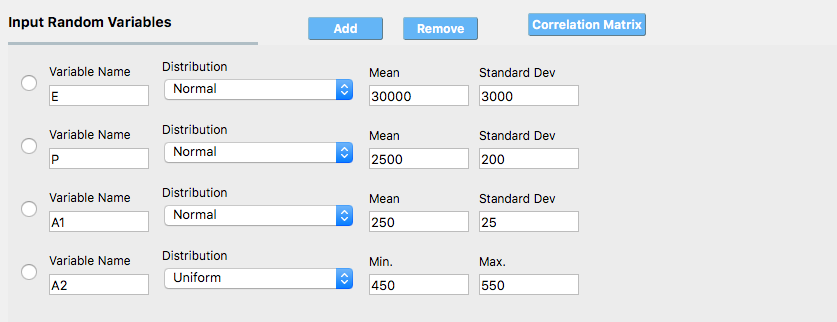
\includegraphics[width=0.8\textwidth]
    {examples/fig_quofem/rv.png} }
  \caption{Random Variable specification}
  \label{fig:rv}
\end{figure}


